\documentclass[]{article}
\usepackage{lmodern}
\usepackage{amssymb,amsmath}
\usepackage{ifxetex,ifluatex}
\usepackage{fixltx2e} % provides \textsubscript
\ifnum 0\ifxetex 1\fi\ifluatex 1\fi=0 % if pdftex
  \usepackage[T1]{fontenc}
  \usepackage[utf8]{inputenc}
\else % if luatex or xelatex
  \ifxetex
    \usepackage{mathspec}
  \else
    \usepackage{fontspec}
  \fi
  \defaultfontfeatures{Ligatures=TeX,Scale=MatchLowercase}
\fi
% use upquote if available, for straight quotes in verbatim environments
\IfFileExists{upquote.sty}{\usepackage{upquote}}{}
% use microtype if available
\IfFileExists{microtype.sty}{%
\usepackage{microtype}
\UseMicrotypeSet[protrusion]{basicmath} % disable protrusion for tt fonts
}{}
\usepackage[margin=1in]{geometry}
\usepackage{hyperref}
\hypersetup{unicode=true,
            pdfborder={0 0 0},
            breaklinks=true}
\urlstyle{same}  % don't use monospace font for urls
\usepackage{color}
\usepackage{fancyvrb}
\newcommand{\VerbBar}{|}
\newcommand{\VERB}{\Verb[commandchars=\\\{\}]}
\DefineVerbatimEnvironment{Highlighting}{Verbatim}{commandchars=\\\{\}}
% Add ',fontsize=\small' for more characters per line
\usepackage{framed}
\definecolor{shadecolor}{RGB}{248,248,248}
\newenvironment{Shaded}{\begin{snugshade}}{\end{snugshade}}
\newcommand{\KeywordTok}[1]{\textcolor[rgb]{0.13,0.29,0.53}{\textbf{{#1}}}}
\newcommand{\DataTypeTok}[1]{\textcolor[rgb]{0.13,0.29,0.53}{{#1}}}
\newcommand{\DecValTok}[1]{\textcolor[rgb]{0.00,0.00,0.81}{{#1}}}
\newcommand{\BaseNTok}[1]{\textcolor[rgb]{0.00,0.00,0.81}{{#1}}}
\newcommand{\FloatTok}[1]{\textcolor[rgb]{0.00,0.00,0.81}{{#1}}}
\newcommand{\ConstantTok}[1]{\textcolor[rgb]{0.00,0.00,0.00}{{#1}}}
\newcommand{\CharTok}[1]{\textcolor[rgb]{0.31,0.60,0.02}{{#1}}}
\newcommand{\SpecialCharTok}[1]{\textcolor[rgb]{0.00,0.00,0.00}{{#1}}}
\newcommand{\StringTok}[1]{\textcolor[rgb]{0.31,0.60,0.02}{{#1}}}
\newcommand{\VerbatimStringTok}[1]{\textcolor[rgb]{0.31,0.60,0.02}{{#1}}}
\newcommand{\SpecialStringTok}[1]{\textcolor[rgb]{0.31,0.60,0.02}{{#1}}}
\newcommand{\ImportTok}[1]{{#1}}
\newcommand{\CommentTok}[1]{\textcolor[rgb]{0.56,0.35,0.01}{\textit{{#1}}}}
\newcommand{\DocumentationTok}[1]{\textcolor[rgb]{0.56,0.35,0.01}{\textbf{\textit{{#1}}}}}
\newcommand{\AnnotationTok}[1]{\textcolor[rgb]{0.56,0.35,0.01}{\textbf{\textit{{#1}}}}}
\newcommand{\CommentVarTok}[1]{\textcolor[rgb]{0.56,0.35,0.01}{\textbf{\textit{{#1}}}}}
\newcommand{\OtherTok}[1]{\textcolor[rgb]{0.56,0.35,0.01}{{#1}}}
\newcommand{\FunctionTok}[1]{\textcolor[rgb]{0.00,0.00,0.00}{{#1}}}
\newcommand{\VariableTok}[1]{\textcolor[rgb]{0.00,0.00,0.00}{{#1}}}
\newcommand{\ControlFlowTok}[1]{\textcolor[rgb]{0.13,0.29,0.53}{\textbf{{#1}}}}
\newcommand{\OperatorTok}[1]{\textcolor[rgb]{0.81,0.36,0.00}{\textbf{{#1}}}}
\newcommand{\BuiltInTok}[1]{{#1}}
\newcommand{\ExtensionTok}[1]{{#1}}
\newcommand{\PreprocessorTok}[1]{\textcolor[rgb]{0.56,0.35,0.01}{\textit{{#1}}}}
\newcommand{\AttributeTok}[1]{\textcolor[rgb]{0.77,0.63,0.00}{{#1}}}
\newcommand{\RegionMarkerTok}[1]{{#1}}
\newcommand{\InformationTok}[1]{\textcolor[rgb]{0.56,0.35,0.01}{\textbf{\textit{{#1}}}}}
\newcommand{\WarningTok}[1]{\textcolor[rgb]{0.56,0.35,0.01}{\textbf{\textit{{#1}}}}}
\newcommand{\AlertTok}[1]{\textcolor[rgb]{0.94,0.16,0.16}{{#1}}}
\newcommand{\ErrorTok}[1]{\textcolor[rgb]{0.64,0.00,0.00}{\textbf{{#1}}}}
\newcommand{\NormalTok}[1]{{#1}}
\usepackage{longtable,booktabs}
\usepackage{graphicx,grffile}
\makeatletter
\def\maxwidth{\ifdim\Gin@nat@width>\linewidth\linewidth\else\Gin@nat@width\fi}
\def\maxheight{\ifdim\Gin@nat@height>\textheight\textheight\else\Gin@nat@height\fi}
\makeatother
% Scale images if necessary, so that they will not overflow the page
% margins by default, and it is still possible to overwrite the defaults
% using explicit options in \includegraphics[width, height, ...]{}
\setkeys{Gin}{width=\maxwidth,height=\maxheight,keepaspectratio}
\IfFileExists{parskip.sty}{%
\usepackage{parskip}
}{% else
\setlength{\parindent}{0pt}
\setlength{\parskip}{6pt plus 2pt minus 1pt}
}
\setlength{\emergencystretch}{3em}  % prevent overfull lines
\providecommand{\tightlist}{%
  \setlength{\itemsep}{0pt}\setlength{\parskip}{0pt}}
\setcounter{secnumdepth}{0}
% Redefines (sub)paragraphs to behave more like sections
\ifx\paragraph\undefined\else
\let\oldparagraph\paragraph
\renewcommand{\paragraph}[1]{\oldparagraph{#1}\mbox{}}
\fi
\ifx\subparagraph\undefined\else
\let\oldsubparagraph\subparagraph
\renewcommand{\subparagraph}[1]{\oldsubparagraph{#1}\mbox{}}
\fi

%%% Use protect on footnotes to avoid problems with footnotes in titles
\let\rmarkdownfootnote\footnote%
\def\footnote{\protect\rmarkdownfootnote}

%%% Change title format to be more compact
\usepackage{titling}

% Create subtitle command for use in maketitle
\newcommand{\subtitle}[1]{
  \posttitle{
    \begin{center}\large#1\end{center}
    }
}

\setlength{\droptitle}{-2em}

  \title{}
    \pretitle{\vspace{\droptitle}}
  \posttitle{}
    \author{}
    \preauthor{}\postauthor{}
    \date{}
    \predate{}\postdate{}
  

\begin{document}

\section*{Conclusion}\label{conclusion}
\addcontentsline{toc}{section}{Conclusion}

\setcounter{chapter}{4} \setcounter{section}{0}

Idea de Rosario -ver dell cluster de saxitoxin cuantos pasos se
necesitron para llegar ahi.\\
-A donde se iria el resultado de abrir el GMP\\
-Otra vez, que Actinos tienen FolE

\subsection{Discusion}\label{discusion}

Finalmente, una pregunta abierta es aún dada una enzima promiscua es la
población promiscua, y son sólo unos confórmeros o todas y cada una de
las enzimas son promiscuas

If we don't want Conclusion to have a chapter number next to it, we can
add the \texttt{\{.unnumbered\}} attribute. This has an unintended
consequence of the sections being labeled as 3.6 for example though
instead of 4.1. The \LaTeX~commands immediately following the Conclusion
declaration get things back on track.

\paragraph{More info}\label{more-info}

And here's some other random info: the first paragraph after a chapter
title or section head \emph{shouldn't be} indented, because indents are
to tell the reader that you're starting a new paragraph. Since that's
obvious after a chapter or section title, proper typesetting doesn't add
an indent there.

\appendix

\section{The First Appendix}\label{the-first-appendix}

This first appendix includes all of the R chunks of code that were
hidden throughout the document (using the \texttt{include\ =\ FALSE}
chunk tag) to help with readibility and/or setup.

\paragraph{In the main Rmd file:}\label{in-the-main-rmd-file}

\paragraph{\texorpdfstring{In
\protect\hyperlink{ref_labels}{}:}{In :}}\label{in}

\section{The Second Appendix, Open source code on this
document}\label{the-second-appendix-open-source-code-on-this-document}

\subsection{R markdown}\label{r-markdown}

Thanks to Rmakdown Thesis\\
Apendix one Useful docker commands\\
-Create a new repository\\
\texttt{docker\ build\ .\ -t\ evomining}\\
\texttt{docker\ push\ nselemevomining}

\subsection{Docker}\label{docker}

Restart docker and free all ports\\
\texttt{sudo\ service\ docker\ restart}

list containers\\
\texttt{docker\ ps\ -a}

ssh or bash into a running docker container\\
\texttt{sudo\ docker\ exec\ -i\ -t\ romantic\_brahmagupta\ /bin/bash}
\texttt{docker\ exec\ -it\ \textless{}mycontainer\textgreater{}\ bash}

Stop all containers\\
\texttt{docker\ rm\ \$(docker\ ps\ -a\ -q)}

Remove stopped containers\\
\texttt{docker\ rm\ \$(docker\ ps\ -q\ -f\ status=exited)}

Remove all images\\
\texttt{docker\ rmi\ \$(docker\ images\ -q)}

uninstall docker from ubuntu (Fresh start)\\
\texttt{sudo\ apt-get\ purge\ docker-engine}\\
\texttt{sudo\ apt-get\ autoremove\ -\/-purge\ docker-engine}\\
\texttt{rm\ -rf\ /var/lib/docker} \# This deletes all images,
containers, and volumes

Run Evomining container using nselem/newevomining image\\
\texttt{docker\ run\ -i\ -t\ -v\ /home/nelly/GIT/EvoMining/:/var/www/html/EvoMining/exchange\ -p\ 80:80\ nselem/newevomining\ /bin/bash}

Start evomining inside this container\\
\texttt{perl\ startevomining}

Vizualice a tree\\
\texttt{http://10.10.100.234/EvoMining/cgi-bin/color\_tree.pl?9\&\&/var/www/html/EvoMining/exchange/CyanosBBH\_MiBIG\_DB.faa\_CYANOS}
file 9.new must be on folder volume CyanosBBH\_MiBIG\_DB.faa\_CYANOS

Find a perl module\\
\texttt{perl\ -MList::Util\ -e\textquotesingle{}print\ \$\_\ .\ "\ =\textgreater{}\ "\ .\ \$INC\{\$\_\}\ .\ "\textbackslash{}n"\ for\ keys\ \%INC\textquotesingle{}}
EvoMining notes\\
Gblocks only runs inside folder /var/www/html/EvoMining

\subsection{Git}\label{git}

\texttt{git\ add\ -\/-all}\\
\texttt{git\ commit\ -m\ "Some\ message"}\\
\texttt{git\ push\ -u\ origin\ master}\\
\texttt{git\ clone}

\subsection{Connect GitHub and
DockerHub}\label{connect-github-and-dockerhub}

automated builds The Dockerfile is available to anyone with access to
your Docker Hub repository. Your repository is kept up-to-date with code
changes automatically.

\subsection{Additional resources}\label{additional-resources}

\begin{itemize}
\item
  \emph{Markdown} Cheatsheet -
  \url{https://github.com/adam-p/markdown-here/wiki/Markdown-Cheatsheet}
\item
  \emph{R Markdown} Reference Guide -
  \url{https://www.rstudio.com/wp-content/uploads/2015/03/rmarkdown-reference.pdf}
\item
  Introduction to \texttt{dplyr} -
  \url{https://cran.rstudio.com/web/packages/dplyr/vignettes/introduction.html}
\item
  \texttt{ggplot2} Documentation -
  \url{http://docs.ggplot2.org/current/}
\end{itemize}

Docker antiSMASH run\_antismash /.gbk \textasciitilde{}/as\_results
--knownclusterblast --inclusive --cf\_threshold 0.7

\section{El tercer Apéndice, Protocolos experimentales utilizados en el
estudio de
PriA}\label{el-tercer-apendice-protocolos-experimentales-utilizados-en-el-estudio-de-pria}

\subsection{Materials}\label{materials}

-Incubator\\
-Refrigerated centrifuge\\
-Sonicator\\
-Column HisTrapHP\\
-Column AKTA-FPLC\\
-Column Vivapure mini\\
-Fluorimeter

\subsection{Purification}\label{purification}

TrpC and TrpD will be purified by Nickel chromatography using AKTA-FPLC
while ScoePriA and D11A purification will be done by Nickel
chromatography using vivapure columns

\subsubsection{Centrifugation}\label{centrifugation}

\begin{enumerate}
\def\labelenumi{\arabic{enumi}.}
\tightlist
\item
  Centrifuge on \(.5L\) cans (Cans as big as possible)\\
  rotor that suits for cans (On \(.5L\) cans rotor code is 03)\\
  Karina: velocity \(6000 rpm\) Time \(10 min\) Ana: \(7000rpm\) for
  \(10 min\) At this point experiment may be interrupted and pellet can
  be stored at \(-80^{\circ}\) on Falcon tubes or better run the essay
  the same day.
\end{enumerate}

To restart this protocol re suspend pellet on \(25 ml\) lysis buffer
keeping on ice all the following steps.

\subsubsection{Sonication}\label{sonication}

We sonicate pellet to disrupt cells and get the proteins. All reactives
must be cooled previously and kept on ice. The sonicator must touch the
falcon tube. Falcon must be kept on ice.

Add fresh components to Lysis buffer:\\
-Add proteasas inhibitor mix \(2\mu l\) (Protein Box)\\
-Add DTT \(.1 25\mu l\)\\
-Karina: Add Lysozyme \(\frac{2mg}{ml}\) \(100\mu l\)\\
-Ana: Add Lysozyme \(\frac{10mg}{ml}\)(\(1000X\)) \(100\mu l\)

\begin{enumerate}
\def\labelenumi{\arabic{enumi}.}
\setcounter{enumi}{1}
\item
  Resuspension. Add lysis Buffer \(25ml\) to resuspend pellet and put
  test tubes on an small glass ware with ice
\item
  Sonication. After buffer addition sonicate:\\
  \(7\) times sonication \(20s\) with \(1min\) rest between every
  sonication cycle.\\
  Only total time of sonication must be entered on sonicaction device
  (\(140s\)).
\item
  Centrifugation. After sonication centrifuge on refrigerated centrifuge
  at 4°C \(25 min\) at \(8000 rpm\)
\item
  Inject into AKTA-FPL previously balanced with Buffer A (or vivapure
  balanced with bufferA)\\
  When vivapure is being used, the supernatant must be filtered on .45
  \(\mu l\) filters to avoid column damage.
\item
  Wash with 5\% Buffer B and subsequently with an imidazol gradient
  (Buffer B) from 5\% to 60\% on 16 vol of the column with a flux of
  1ml/min. Conserve each elution tube properly labeled. 2000rpm 5 min\\
  What we did to purificate Scoe PriA was an imidazol gradient:
\end{enumerate}

Flask each one with a 100ml were prepared. columns were washed with 20ml
of this tubes at 2000rpm 5 min\\
Imidazol concentration=x\\
v: (x=)100ml/500mM

\label{my-label enzyme}

\begin{tabular}{ l l c c l}
\hline \\ [-1.5ex]
Flask & BufferB (mM)   & BufferB (ml)  & Buffer A ml & Buffer B  \\  [1ex]
\hline \\ [-1.5ex]
1 & 50& 10&  90& 10 \\  [1ex]
2 & 100& 20& 80& 20 \\  [1ex]
3 & 150& 30& 70 & 30 \\  [1ex]
4 & 300& 60& 40 & 60 \\  [1ex]
5 & 500& 100& 0& 100 \\  [1ex]
\hline
\end{tabular}

Flask must be ketp cold.

\begin{enumerate}
\def\labelenumi{\arabic{enumi}.}
\setcounter{enumi}{6}
\item
  Recover the fractions that contains the protein that elutes
  approximately at 150-200 mM imidazol. (TrpC, TrpD) or 300mM imidazol
  (must PriA). Collect the relevant fractions. At this point a protein
  gel can be run to check protein elution.
\item
  Concentrate the protein using AMICON tubes 10kDa (all molecules below
  this weight will be discarded, molecules with weight above 10kDa such
  as PriA will be kept inside the tube) until an approximate
  concentration of \(90 \frac{\mu g}{\mu l}\) (\(1ml\) vol approx).
  Because imidazol\textgreater{}200mM reacts with Bradford, protein on
  amicon must be washed with 10 ml of buffer A to eliminate imidazol
  (4ml each time on amicon tube). Finally, after protein concentration,
  100 ul sample must be recovered with 900 ul Buffer A (free of
  imidazol) (8000 rpm 10 min) when AMICON are stored for long periods
  leave on ethanol at 20\%, to reuse them throw ethanol out and wash
  many times with miliQ water.
\item
  Check purity by SDS-PAGE gel\\
  on \emph{S coelicolor} PriA molecular weight is around 25.7 kDa
  (length 240 aminoacids), on \emph{T maritima} TrpC molecular weight is
  around 27.5 kDa (length 242 aminoacids)
\item
  Add glycerol at a final concentration of 15\% and quantify using
  Bradford. Store at -80C
\end{enumerate}

\emph{TrpC important before step 5}\\
After centrifuge step 4 :\\
Heat supernatant by 15 min at 65C\\
Centrifuge at 10000rpm by 20min. Recover the supernatant.

Continue with steps 5-10 as in trpD purification.

On protein activity is more important to be pure than to have protein
abundance.

\subsection{Protein Quantification}\label{protein-quantification}

\subsubsection{Bradford calibration
curve}\label{bradford-calibration-curve}

Mix well while pipeting. Holes with protein content must become blue.\\
Incubate 5 min.\\
Measure at 595 abs (TECAN). clear box.\\
5 ul y 50ul of protein. Take measures inside the curve range.\\
BSA on ug/ml

\$\$ \label{ScoD11_A}

\begin{tabular}{c c c c}
\hline 
BSA $\mu l$ por ml & BSA $\mu l$ & Bradford $\mu l$ & Other \\ [1ex]
\hline \\ [-1.5ex]  
0                & 0      & 40 & $H_2O$ 160 $\mu l$   \\ [1 ex]
10               & 160    & 40 &    -                 \\ [1 ex]
20               & 160    & 40 & -                    \\ [1 ex]
40               & 160    & 40 & -                    \\ [1 ex]
60               & 160    & 40 &-                     \\ [1 ex]
100              & 160    & 40 & -                    \\ [1 ex]
0                &   0    & 40 &  PriA 5 $\mu l$   $H_2O$ 155 $\mu l$   \\ [1 ex]
0                &   0    & 40 &  PriA 20 $\mu l$   $H_2O$ 130 $\mu l$  \\ [1 ex]

\hline  
\end {tabular}

\$\$

\begin{Shaded}
\begin{Highlighting}[]
\NormalTok{## 160 ul of BSA on this concentrations on ug/ml were added to a 40 ul of Bradford}
\NormalTok{##BSA concentration on ug/ml}
\NormalTok{BSAConcentrationStock<-}\KeywordTok{c}\NormalTok{(}\DecValTok{0}\NormalTok{,}\DecValTok{10}\NormalTok{,}\DecValTok{20}\NormalTok{,}\DecValTok{40}\NormalTok{,}\DecValTok{60}\NormalTok{,}\DecValTok{100}\NormalTok{)}

\CommentTok{#adding .16 ml on plates  }
\NormalTok{vol<-}\DecValTok{160}
\NormalTok{Bradford_df =}\StringTok{ }\KeywordTok{data.frame}\NormalTok{(BSAConcentrationStock,vol)   }

\NormalTok{## quantity of microgrames on .16 ml}
\NormalTok{Bradford_df[}\StringTok{"Quantity"}\NormalTok{]<-BSAConcentrationStock*.}\DecValTok{160}
\NormalTok{## concentration after added 40 ul bradford (total 200 ul)}
\NormalTok{Bradford_df[}\StringTok{"Concentration200"}\NormalTok{]<-Bradford_df[}\StringTok{"Quantity"}\NormalTok{]/.}\DecValTok{2}


\NormalTok{## This are the absorbance measures for the different BSA concentrations  }
\NormalTok{Abs1BSA<-}\KeywordTok{c}\NormalTok{(}\FloatTok{0.2649999857}\NormalTok{,}\FloatTok{0.4329000115}\NormalTok{,}\FloatTok{0.6754000187}\NormalTok{,}\FloatTok{0.9449999928}\NormalTok{,}\FloatTok{1.24240005}\NormalTok{,}\FloatTok{1.432000041}\NormalTok{)}
\NormalTok{Abs2BSA<-}\KeywordTok{c}\NormalTok{(}\FloatTok{0.2948000133}\NormalTok{,}\FloatTok{0.4298999906}\NormalTok{,}\FloatTok{0.7348999977}\NormalTok{,}\FloatTok{0.9965000153}\NormalTok{,}\FloatTok{1.225999951}\NormalTok{,}\FloatTok{1.494899988}\NormalTok{)}

\NormalTok{Bradford_df[}\StringTok{"Abs1BSA"}\NormalTok{]<-Abs1BSA}
\NormalTok{Bradford_df[}\StringTok{"Abs2BSA"}\NormalTok{]<-Abs2BSA}

\NormalTok{## mean value of measures}
\NormalTok{Bradford_df$mean<-}\KeywordTok{rowMeans}\NormalTok{(}\KeywordTok{subset}\NormalTok{(Bradford_df, }\DataTypeTok{select =} \KeywordTok{c}\NormalTok{(Abs1BSA, Abs2BSA)), }\DataTypeTok{na.rm =} \OtherTok{TRUE}\NormalTok{)}

\CommentTok{#adjusting blank}
\NormalTok{Bradford_df$meanAdjusted<-Bradford_df$mean-Bradford_df$mean[}\DecValTok{1}\NormalTok{]}
\NormalTok{BSA.lm =}\StringTok{ }\KeywordTok{lm}\NormalTok{(meanAdjusted ~}\StringTok{ }\NormalTok{Concentration200, }\DataTypeTok{data=}\NormalTok{Bradford_df) }
\NormalTok{coeffs =}\StringTok{ }\KeywordTok{coefficients}\NormalTok{(BSA.lm); coeffs }
\end{Highlighting}
\end{Shaded}

\begin{verbatim}
##      (Intercept) Concentration200 
##       0.10688027       0.01502265
\end{verbatim}

\begin{Shaded}
\begin{Highlighting}[]
\NormalTok{b=coeffs[}\DecValTok{1}\NormalTok{]}
\NormalTok{m=coeffs[}\DecValTok{2}\NormalTok{]}

\NormalTok{eq =}\StringTok{ }\NormalTok{function(x)\{x*m+b\}}
\KeywordTok{plot}\NormalTok{(Bradford_df$Concentration200,Bradford_df$meanAdjusted,}\DataTypeTok{type=}\StringTok{"l"}\NormalTok{)}
\KeywordTok{par}\NormalTok{(}\DataTypeTok{new=}\OtherTok{TRUE}\NormalTok{)}
\KeywordTok{plot}\NormalTok{(eq, }\DecValTok{1}\NormalTok{,}\DecValTok{100}\NormalTok{)}
\end{Highlighting}
\end{Shaded}

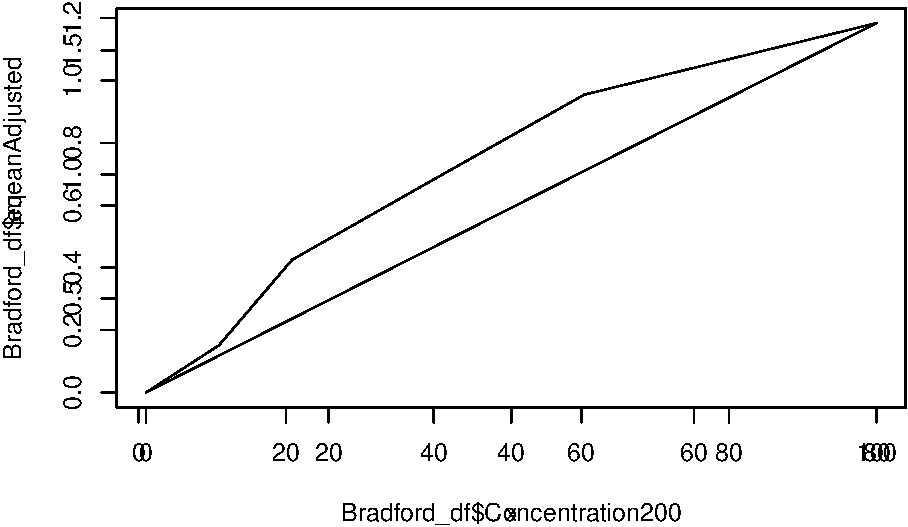
\includegraphics{conclusion_files/figure-latex/BSA_Bradford-1.pdf}

\subsubsection{Enzyme quantification}\label{enzyme-quantification}

For Bradford to work properly After protein concentration, 900 ul Buffer
A (free of imidazol) must be added to 100 \(\mu l\) sample

\begin{Shaded}
\begin{Highlighting}[]
\NormalTok{##  ul of }
\NormalTok{vol=}\DecValTok{5}
\NormalTok{type=}\StringTok{"Scoe"}
\NormalTok{ABS1=}\FloatTok{0.932099998}    
\NormalTok{ABS2=}\FloatTok{1.048400044}
\NormalTok{Pria_df=}\KeywordTok{data.frame}\NormalTok{(vol,type,ABS1,ABS2)}
\NormalTok{Pria_df$type<-}\KeywordTok{as.character}\NormalTok{(Pria_df$type)}
\NormalTok{data2=}\KeywordTok{c}\NormalTok{(}\DecValTok{20}\NormalTok{,}\StringTok{"Scoe"}\NormalTok{,}\FloatTok{1.639400005}\NormalTok{,}\FloatTok{1.569700003}\NormalTok{)}
\NormalTok{data3=}\KeywordTok{c}\NormalTok{(}\DecValTok{5}\NormalTok{,}\StringTok{"D11A"}\NormalTok{,}\FloatTok{0.575600028}\NormalTok{,   }\FloatTok{0.576099992}\NormalTok{)}
\NormalTok{data4=}\KeywordTok{c}\NormalTok{(}\DecValTok{20}\NormalTok{,}\StringTok{"D11A"}\NormalTok{,}\FloatTok{1.039499998}\NormalTok{,  }\FloatTok{1.067399979}\NormalTok{)}
\NormalTok{data5=}\KeywordTok{c}\NormalTok{(}\DecValTok{160}\NormalTok{,}\StringTok{"test"}\NormalTok{,.}\DecValTok{69085}\NormalTok{,  .}\DecValTok{69085}\NormalTok{)}

\NormalTok{## add data to dataframe Pria_df}
\NormalTok{Pria_df=}\KeywordTok{rbind}\NormalTok{(Pria_df,data2)}
\NormalTok{Pria_df=}\KeywordTok{rbind}\NormalTok{(Pria_df,data3)}
\NormalTok{Pria_df=}\KeywordTok{rbind}\NormalTok{(Pria_df,data4)}
\NormalTok{Pria_df=}\KeywordTok{rbind}\NormalTok{(Pria_df,data5)}

\NormalTok{Pria_df$mean<-}\KeywordTok{rowMeans}\NormalTok{(}\KeywordTok{cbind}\NormalTok{(}\KeywordTok{as.numeric}\NormalTok{(Pria_df$ABS1),}\KeywordTok{as.numeric}\NormalTok{(Pria_df$ABS2)))}

\NormalTok{## Pasando absorbancia a concentration de proteina en 200 ul (ug/ml)}
\NormalTok{## kari values }
\CommentTok{#m=0.004679534923}
\CommentTok{#b=0.103674687}

\NormalTok{inter =}\StringTok{ }\NormalTok{function(y)\{(y-b)/m\}}
\NormalTok{Pria_df$concentration200<-}\KeywordTok{inter}\NormalTok{(Pria_df$mean)}

\NormalTok{## protein quantity on ug on 200 ul}
\NormalTok{Pria_df[}\StringTok{"Quantity"}\NormalTok{]=Pria_df$concentration200*.}\DecValTok{2}

\NormalTok{### Inicial concentration  C200_vol200=Cinicial_Vinicial}
\NormalTok{Pria_df[}\StringTok{"ConcentrationInitial"}\NormalTok{]=Pria_df$Quantity/(.}\DecValTok{001}\NormalTok{*}\KeywordTok{as.numeric}\NormalTok{(Pria_df$vol))}

\KeywordTok{kable}\NormalTok{(Bradford_df)}
\end{Highlighting}
\end{Shaded}

\begin{longtable}[]{@{}rrrrrrrr@{}}
\toprule
BSAConcentrationStock & vol & Quantity & Concentration200 & Abs1BSA &
Abs2BSA & mean & meanAdjusted\tabularnewline
\midrule
\endhead
0 & 160 & 0.0 & 0 & 0.2650 & 0.2948 & 0.27990 & 0.00000\tabularnewline
10 & 160 & 1.6 & 8 & 0.4329 & 0.4299 & 0.43140 & 0.15150\tabularnewline
20 & 160 & 3.2 & 16 & 0.6754 & 0.7349 & 0.70515 & 0.42525\tabularnewline
40 & 160 & 6.4 & 32 & 0.9450 & 0.9965 & 0.97075 & 0.69085\tabularnewline
60 & 160 & 9.6 & 48 & 1.2424 & 1.2260 & 1.23420 & 0.95430\tabularnewline
100 & 160 & 16.0 & 80 & 1.4320 & 1.4949 & 1.46345 &
1.18355\tabularnewline
\bottomrule
\end{longtable}

\begin{Shaded}
\begin{Highlighting}[]
\KeywordTok{kable}\NormalTok{(Pria_df)}
\end{Highlighting}
\end{Shaded}

\begin{longtable}[]{@{}llllrrrr@{}}
\toprule
vol & type & ABS1 & ABS2 & mean & concentration200 & Quantity &
ConcentrationInitial\tabularnewline
\midrule
\endhead
5 & Scoe & 0.932099998 & 1.048400044 & 0.99025 & 58.80251 & 11.760502 &
2352.10030\tabularnewline
20 & Scoe & 1.639400005 & 1.569700003 & 1.60455 & 99.69408 & 19.938816 &
996.94081\tabularnewline
5 & D11A & 0.575600028 & 0.576099992 & 0.57585 & 31.21750 & 6.243500 &
1248.70007\tabularnewline
20 & D11A & 1.039499998 & 1.067399979 & 1.05345 & 63.00948 & 12.601897 &
630.09485\tabularnewline
160 & test & 0.69085 & 0.69085 & 0.69085 & 38.87261 & 7.774521 &
48.59076\tabularnewline
\bottomrule
\end{longtable}

Since 1kDa = 1Kg/mol and PriA Scoe molecular weight is 25.7kDa we have
that\\
\(M\times V = \frac{g}{mw}\)\\
\(M=\frac{g}{V}\times\frac{1}{mw}\)

\begin{Shaded}
\begin{Highlighting}[]
\NormalTok{## mas on Kda = kg/mol  }
\NormalTok{mw<-}\FloatTok{25.7} 
\CommentTok{# converting to g/mol  }
\NormalTok{mwgram<-mw*}\DecValTok{1000}  
\NormalTok{## concentration on g/L (after convert ug/ml)}
\NormalTok{concentScoe<-}\FloatTok{2.352}
\NormalTok{concentD11A<-}\FloatTok{1.248}
\NormalTok{## Concentration on uM (10**6M)}
\NormalTok{molar =}\StringTok{ }\NormalTok{function(x)\{(}\DecValTok{10}\NormalTok{**}\DecValTok{6}\NormalTok{)*x/mwgram\}}
\KeywordTok{molar}\NormalTok{(concentScoe)}
\end{Highlighting}
\end{Shaded}

\begin{verbatim}
## [1] 91.51751
\end{verbatim}

\begin{Shaded}
\begin{Highlighting}[]
\KeywordTok{molar}\NormalTok{(concentD11A)}
\end{Highlighting}
\end{Shaded}

\begin{verbatim}
## [1] 48.56031
\end{verbatim}

\subsection{Concentration on
microMolar}\label{concentration-on-micromolar}

\begin{quote}
So Scoe concentration is 91.5175097 and D11A is 48.5603113 \(\mu M\)
\end{quote}

\begin{Shaded}
\begin{Highlighting}[]
\NormalTok{## we want final concentration 2.4uM on a final volume of 160 ul}
\NormalTok{## ciVi=CfVf}
\NormalTok{## Vi =CfVf/Vi}
\NormalTok{## Cf= 80uM Vf=5ul Vi=?ul Ci=x}

\NormalTok{adjustMol =}\StringTok{ }\NormalTok{function(x)\{}\FloatTok{2.5}\NormalTok{*}\DecValTok{160}\NormalTok{/x\} }
\NormalTok{## this are the ul need from stock cristal enzyme that will be diluted on buffer to complete 160 ul }
\KeywordTok{adjustMol}\NormalTok{(}\KeywordTok{molar}\NormalTok{(concentScoe))}
\end{Highlighting}
\end{Shaded}

\begin{verbatim}
## [1] 4.370748
\end{verbatim}

\begin{Shaded}
\begin{Highlighting}[]
\KeywordTok{adjustMol}\NormalTok{(}\KeywordTok{molar}\NormalTok{(concentD11A))}
\end{Highlighting}
\end{Shaded}

\begin{verbatim}
## [1] 8.237179
\end{verbatim}


\end{document}
